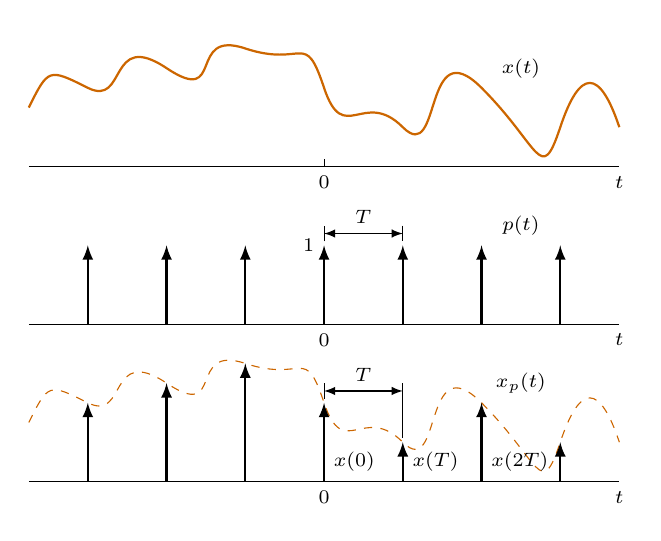
\begin{tikzpicture}[x=0.5cm, y=0.5cm]
	\draw (-7.5, 0) -- (7.5, 0) node [anchor=north] {\scriptsize $t$};
	\draw (0,0) -- ++(0,0.2);
	\node at (0,0)  [anchor=north] {\scriptsize $0$};
	\draw [thick, orange!80!black]
	(-7.5,1.5)
	.. controls (-7,2.5) and (-7,2.5) .. (-6,2)
	.. controls (-5,1.5) and (-5.5,3.5) .. (-4,2.5)
	.. controls (-2.5,1.5) and (-3.5,3.5) .. (-2,3)
	.. controls (-0.5,2.5) and (-0.5,3.5) .. (0,2)
	.. controls (0.5,0.5) and (1,2) .. (2,1)
	.. controls (3,0) and (2.5,3.5) .. (4,2)
	.. controls (5.5,0.5) and (5.5,-0.5) .. (6,1)
	.. controls (6.5,2.5) and (7,2.5) .. (7.5,1);	
	\node at (5,2)  [anchor=south] {\scriptsize $x(t)$};

\pause
\begin{scope}[yshift=-2cm]
	\draw (-7.5, 0) -- (7.5, 0) node [anchor=north] {\scriptsize $t$};	
	\node at (0,0)  [anchor=north] {\scriptsize $0$};	
	\foreach \i/\s in {-6/{-3T}, -4/{-2T}, -2/{-T}, 0/0, 2/{T}, 4/{2T}, 6/{3T} }
	{
		\draw[-latex, thick] (\i, 0) -- ++(0, 2);
	}
	\node at (5,2)  [anchor=south] {\scriptsize $p(t)$};	
	\node at (0,2)  [anchor=east] {\scriptsize $1$};	
	\draw (0, 2.1) -- ++(0, 0.4) ++(0, -0.2)  ++(2,0)   ++(0, 0.2) -- ++(0, -0.4) ;
	\draw[latex-latex] (0, 2.3) -- ++(2,0)  node[midway, above] {\scriptsize $T$};
\end{scope}

\pause
\begin{scope}[yshift=-4cm]
	\draw (-7.5, 0) -- (7.5, 0) node [anchor=north] {\scriptsize $t$};	
	\node at (0,0)  [anchor=north] {\scriptsize $0$};	
	\draw [orange!80!black, dashed]
	(-7.5,1.5)
	.. controls (-7,2.5) and (-7,2.5) .. (-6,2)
	.. controls (-5,1.5) and (-5.5,3.5) .. (-4,2.5)
	.. controls (-2.5,1.5) and (-3.5,3.5) .. (-2,3)
	.. controls (-0.5,2.5) and (-0.5,3.5) .. (0,2)
	.. controls (0.5,0.5) and (1,2) .. (2,1)
	.. controls (3,0) and (2.5,3.5) .. (4,2)
	.. controls (5.5,0.5) and (5.5,-0.5) .. (6,1)
	.. controls (6.5,2.5) and (7,2.5) .. (7.5,1);	
	\foreach \i/\s in {-6/{2}, -4/{2.5}, -2/{3}, 0/2, 2/{1}, 4/{2}, 6/{1} }
	{
		\draw[-latex, thick] (\i, 0) -- ++(0, \s);
	}
	\node at (5,2)  [anchor=south] {\scriptsize $x_p(t)$};	
	\draw (0, 2.1) -- ++(0, 0.4) ++(0, -0.2)  ++(2,0)   ++(0, 0.2) -- ++(0, -1.4) ;
	\draw[latex-latex] (0, 2.3) -- ++(2,0)  node[midway, above] {\scriptsize $T$};
	\node at (0,0.5) 	 [anchor=west] {\scriptsize $x(0)$};
	\node at (2,0.5) 	 [anchor=west] {\scriptsize $x(T)$};
	\node at (4,0.5) 	 [anchor=west] {\scriptsize $x(2T)$};	
\end{scope}
\end{tikzpicture} 